\documentclass[manuscript, screen, review]{jair}

\setcopyright{cc}

\JAIRTrack{}

\acmDOI{10.1613/jair.1.xxxxx}

\RequirePackage[
  datamodel=acmdatamodel,
  style=acmauthoryear,
  backend=biber,
  giveninits=true,
  uniquename=init
]{biblatex}

\renewcommand*{\bibopenbracket}{(}
\renewcommand*{\bibclosebracket}{)}

\addbibresource{references.bib}

\begin{document}

\title[Automatic Prioritization of IT Support Tickets]
{Automatic Prioritization of IT Support Tickets Using Natural Language Processing and Explainable AI: A Data-Driven Evaluation of Machine Learning Classifiers Based on the CRISP-DM Model}

\author{Verena Gräf}

\email{xverenagraefx@gmail.com}

\affiliation{%
  \institution{FOM University of Applied Sciences}
  \city{Bonn}
  \country{Germany}
}

\renewcommand{\shortauthors}{Gräf}

\begin{abstract}
{\bf Background:}
Determining the priority of IT support tickets dictates the order of requests with different urgency levels, which is particularly important for time-critical cases. Since this decision is largely guided by unstructured
ticket descriptions, automation using Natural Language Processing (NLP) offers potential for automated support.

{\bf Objectives:}
The study investigated different machine learning classifiers concerning classification performance and explainability for NLP-based ticket prioritization.


{\bf Methods:}
The classifier comparison used a publicly available, synthetically generated IT support ticket dataset, with Macro-F1 as the performance metric. Differences in performance relative to a Logistic Regression baseline were assessed using paired bootstrap resampling with Holm correction. Finally, explainability was
operationalized by measuring the concentration of absolute SHapley Additive exPlanations (SHAP) attributions.

{\bf Results:}
On the common feature set, LightGBM showed the highest hold-out performance and significantly outperformed Logistic Regression by 0.0197 Macro-F1 points ($p_{\mathrm{Holm}} = 0.024$). The final LightGBM model selected using cross-validation achieved a hold-out Macro-F1 of 0.5597. Logistic Regression showed significantly more concentrated SHAP attributions than Complement Naive Bayes ($\Delta = 0.0775$) and Random Forest ($\Delta = 0.0741$). Both comparisons were significant after Holm correction
($p_{\mathrm{Holm}} < 0.001$). However, no superiority over all alternative classifiers could be shown.

{\bf Conclusions:}
The results suggest that classification performance and SHAP-based explanation properties constitute different dimensions of the prioritization task and should therefore be evaluated independently during model selection.

\end{abstract}

\maketitle

\section{Introduction}

In IT Service Management (ITSM), the prioritization of IT support tickets determines the order in which requests are processed by assigning them to priority levels according to their urgency and business impact. In practice, this assessment is often performed by support staff based on the problem description contained in the ticket \cite{lyubinets2018labeling,razma2026classification}.

Relying on text for this decision creates opportunities to automate the prioritization process. Machine learning (ML) classifiers predict the priority class of tickets, while unstructured ticket descriptions are preprocessed using Natural Language Processing (NLP) techniques \cite{lyubinets2018labeling,braun-2026-solving,selvi2025customer}. This supports manual evaluation and automates priority assignment \cite{braun-2026-solving}.

Recent studies on IT support data show that text-based classification models must address challenges such as multilingual input and imbalanced class distributions under real-world conditions \cite{razma2026classification}. Studies further show that both the choice of classifier and the text representation can affect classification performance \cite{lyubinets2018labeling,revina2020ticket}.

In addition to predictive performance, automated classification decisions raise the question of which information a model relies on when generating its predictions. Explainable Artificial Intelligence (XAI) considers explainability a multidimensional construct \cite{guidotti2018survey,sokol2020factsheets}. \citet{nauta2023evaluation} identify the compactness of an explanation as a distinct and quantitatively assessable property. Shapley additive explanations (SHAP) provide an approach applicable across model types for the attribution-based analysis of individual predictions \cite{lundberg2017shap}.

Although the automated processing of IT support tickets is an established research field, a substantial part of the literature focuses on general ticket classification, routing, and assignment \cite{zangari2023ticket,fuchs2022support}. Explainability has also been investigated in the context of support ticket classification \cite{zicari2022ticket,licina2026helpagent}. However, the combination of a comparative performance benchmark for priority prediction with a cross-model quantitative evaluation of SHAP-based explanation properties has received only limited attention in the literature reviewed for this study. This highlights the need for comparative studies that place priority prediction at the center of the analysis.

Motivated by these gaps, the present study investigates NLP-based priority prediction for IT support tickets using multiple ML classifiers. The following research questions are addressed.

\textbf{RQ1:} How do ML classifiers differ in their classification performance for NLP-based prioritization of IT support tickets?

\textbf{RQ2:} How do the investigated classifiers differ in terms of the SHAP-based explainability of their predictions?

For the performance comparison, Logistic Regression is used as the reference model. Linear, neighborhood-based, tree-based, and ensemble-based methods have been comparatively applied in research on ticket classification \cite{revina2020ticket,fuchs2022support,paramesh2018ensemble}. Studies in the IT support context show that alternative model classes can achieve higher Macro-F1 scores than a Logistic Regression baseline \cite{razma2026classification}. Based on this evidence, the following directional hypothesis is derived for the first research question.

\textbf{H1:} At least one of the investigated alternative classifiers achieves a higher Macro-F1 score than the Logistic Regression baseline for NLP-based prioritization of IT support tickets.

The second research question extends the model comparison by considering SHAP-based explainability. As explainability is a multidimensional construct, the inferential analysis focuses on explanation compactness as a quantitatively assessable dimension \cite{nauta2023evaluation}. While more complex model classes are often regarded as black boxes, linear models are considered easier to interpret due to their transparent decision structure \cite{ribeiro2016lime,lundberg2017shap,guidotti2018survey}. Against this background, the following directional hypothesis is formulated.

\textbf{H2:} At least one of the investigated alternative classifiers exhibits lower SHAP-based explanation compactness than the Logistic Regression baseline.

This study advances automated ticket prioritization research by comparing multiple classifiers under a common data, feature, and evaluation framework and by extending performance evaluation with a quantitative comparison of SHAP-based explanation compactness. This study does not compare different XAI methods, conduct a user-based evaluation, or test the approach in a production environment.

In the following, Section~2 contextualizes the study within the current state of research before Section~3 details the methodological approach. The empirical results are presented in Section~4 and subsequently discussed regarding their broader implications and limitations in Section~5. The paper concludes with Section~6, which summarizes the central findings.
\section{Related Work}

This section reviews the theoretical and empirical foundations of automated IT support ticket prioritization. After positioning ticket prioritization within the broader context of ITSM, it outlines NLP-based feature representations and relevant machine learning classifiers. Finally, XAI is introduced as the foundation for evaluating explainability.

\subsection{Ticket Prioritization in IT Service Management}

Support ticket systems provide a central interface between users and the help desk in ITSM by recording technical problems and service requests as tickets \cite{alhawari2021helpdesk,fuchs2022support}. Tickets typically contain textual problem descriptions as well as additional information such as category or priority \cite{fuchs2022support,zangari2023ticket}. The ticket management process comprises activities such as logging, classification, prioritization, assignment, subsequent processing, and closure \cite{alhawari2021helpdesk}.

Prioritization represents a distinct decision task within ticket processing. In an ITSM context, priority is determined based on criteria such as urgency and business impact \cite{razma2026classification}. This decision is relevant because limited resources require tickets to be processed in a prioritized order and important tickets to be addressed early \cite{tian2015priority}. Tickets may also be subject to time-bound service requirements. Delays can affect business processes, while violations of Service Level Agreements (SLAs) may have financial consequences \cite{gupta2012scheduling}.

Ticket automation covers different tasks such as classification, routing, expert finding, and ticket resolution \cite{fuchs2022support,zangari2023ticket}. Within this broader scope, ticket prioritization constitutes a specific classification task in which incoming tickets are assigned to a priority class \cite{lyubinets2018labeling,beckers2009multifacet}.

\subsection{NLP-Based Feature Representation for Ticket Data}

For automated classification, unstructured ticket texts must be transformed into numerical feature representations. Ticket texts may contain short descriptions, domain-specific terminology, abbreviations, or technical artifacts. Real-world IT support data may additionally involve challenges such as multilingual input and class imbalance \cite{lyubinets2018labeling,razma2026classification}. Beyond the ticket text itself, features derived from the subject line, text position, punctuation, attachments, and sender information can provide relevant information \cite{beckers2009multifacet}.

An established representation for text classification is Term Frequency--Inverse Document Frequency (TF-IDF), which represents documents as high-dimensional, sparse vectors based on weighted terms \cite{manning2008introduction}. TF-IDF is also combined with classical machine learning methods in ticket classification \cite{revina2020ticket}. One limitation is that relationships between terms are captured only to a limited extent \cite{bonechi2024support}.

Contextual language models such as BERT, by contrast, incorporate both left and right linguistic context and can be fine-tuned for downstream classification tasks \cite{devlin2019bert}. Recent ticket studies compare classical TF-IDF-based approaches with transformer-based models \cite{bonechi2024support,razma2026classification}. \citet{bonechi2024support} show that BERT can achieve higher classification performance, whereas TF-IDF combined with Support Vector Machine (SVM) provides a simpler and more resource-efficient alternative.

\subsection{Machine Learning Classifiers for Ticket Prioritization}

Ticket classification has been investigated using different model families, including probabilistic, linear, instance-based, and tree-based methods as well as ensemble, deep learning, and transformer models \cite{revina2020ticket,ahmed2023incident}. Comparative studies indicate that model performance varies depending on the underlying data and classification task, and no uniformly superior model family can be identified across different application contexts \cite{revina2020ticket,ahmed2023incident}. Their respective strengths and limitations for text-based ticket data are therefore particularly relevant for their methodological positioning.

Naive Bayes methods constitute an established probabilistic family for text classification and can be applied efficiently to high-dimensional text data due to their comparatively low computational complexity. Their modeling, however, relies on strong conditional-independence assumptions between features. Limitations may arise particularly in the presence of imbalanced text classes \cite{kibriya2004multinomial,frank2006naive}. Complement Naive Bayes is also used as a comparison method in ticket classification and therefore extends the model comparison by a probabilistic model family \cite{zicari2022ticket}.

For large and sparse feature spaces such as those produced by TF-IDF, Logistic Regression and linear SVMs are particularly suitable, as they learn linear decision functions  \cite{joachims1998text,fan2008liblinear}. This efficiency comes with a limited ability to directly model nonlinear interactions. Nevertheless, recent help desk studies report competitive SVM performance compared with Random Forest, Long Short-Term Memory (LSTM) models, and BERT, in some cases with lower computational resource requirements \cite{martins2024port,bonechi2024support}.

Instead of learning a global decision function, k-Nearest Neighbors (kNN) serves as an instance-based alternative that classifies new instances based on similar training observations \cite{cover1967nearest}. Its performance depends directly on the selected similarity metric and the structure of the feature space. kNN is also used as a comparison method in ticket classification \cite{revina2020ticket}.

Tree-based ensemble methods can model nonlinear relationships and feature interactions. Random Forest aggregates randomized decision trees and thereby reduces dependence on individual tree structures \cite{breiman2001random}. Boosting methods, by contrast, construct models sequentially. XGBoost combines this principle with, among other techniques, regularization and sparsity-aware processing \cite{chen2016xgboost}, whereas LightGBM is specifically designed for efficient gradient boosting on large and high-dimensional datasets \cite{ke2017lightgbm}. This increased model flexibility is accompanied by greater model and tuning complexity.

Recent empirical findings further illustrate the dependence of model performance on the specific application context. In the industrial IT incident data analyzed by \citet{ahmed2023incident}, XGBoost is among the strongest methods on one dataset, whereas convolutional neural networks or transformer models achieve the best results on other subsets. In contrast, \citet{martins2024port} report the highest F1-scores for SVM on real-world help desk requests and substantially shorter training times for classical methods compared with BERT and LSTM. These differing findings provide the rationale for RQ1 and the controlled comparison of multiple model families under a common data, feature, and evaluation basis.

\subsection{Explainable AI and Explanation Quality}

In addition to classification performance, it is relevant to understand the information on which model predictions are based. XAI encompasses approaches intended to make machine learning predictions and model behavior more understandable \cite{guidotti2018survey,arrieta2020xai, adadi2018peeking}. Explainability has also been investigated in the ticket context. \citet{zicari2022ticket} combine ticket classification with local explanation methods to analyze relevant features and misclassifications, whereas \citet{licina2026helpagent} integrate SHAP-based explanations into a help desk system.

Established local explanation methods include Local Interpretable Model-Agnostic Explanations (LIME), which approximates a model's behavior around an individual prediction using an interpretable local surrogate model \cite{ribeiro2016lime}. SHAP, in turn, provides an approach to feature attribution by assigning individual feature contributions to a specific model prediction \cite{lundberg2017shap}. This enables models from different families to be examined based on their attribution patterns. However, explanation quality is multidimensional. \citet{nauta2023evaluation} distinguish twelve properties of explanation quality and include \emph{Compactness} as a separate property concerned with how extensive an
explanation is.

The existing literature therefore includes both diverse approaches to ticket classification and applications of XAI in the ticket context. Although model comparisons focus primarily on classification performance and explanation-oriented studies examine individual XAI applications, cross-model quantitative comparisons of SHAP-based explanation properties in the context of priority prediction remain limited in the reviewed literature. To address this gap, the present study extends the performance comparison in RQ1 with a quantitative assessment of explanation compactness in RQ2.
\section{Methodology}

This section describes the methodological approach of the study. First, the research design and data basis are presented. This is followed by data preparation and feature representation, model development and performance evaluation, and the SHAP-based explainability analysis.

\subsection{Research Design and Data Basis}

The study followed a quantitative, comparative research design and operationalized IT support ticket prioritization as a supervised multiclass classification task with the target classes \textit{low}, \textit{medium}, and \textit{high}. The Cross-Industry Standard Process for Data Mining (CRISP-DM) was used as the process framework, structuring the phases Business Understanding, Data Understanding, Data Preparation, Modeling, and Evaluation \cite{chapman2000crisp}. This study did not include the Deployment phase because no production system integration was conducted. The resulting empirical research workflow is illustrated in Figure~\ref{fig:Pipeline}.

\begin{figure}[ht]
    \centering
    
\includegraphics[width=\linewidth]{figures/Pipeline.png}
    \caption{Investigation model of the empirical analysis for NLP-based prioritization of IT support tickets and SHAP-based explainability analysis.}
    \label{fig:Pipeline}
    \Description{Flow diagram showing the analysis pipeline from the ticket
    dataset through data understanding, preprocessing, semantic grouping,
    train--hold-out splitting, screening, feature-set construction, model training
    and cross-validation, and the subsequent classification-performance and
    SHAP-based explainability analyzes.}
\end{figure}

The publicly available \textit{Customer IT Support Ticket Dataset} by \citet{bueck2025support} served as the data source. The synthetically generated raw dataset comprised 28,587 tickets and 16 variables and was selected because it provides multilingual ticket texts, priority labels, and structured contextual features in a publicly accessible and reproducible form. The modeling input comprised ticket texts derived from \texttt{subject} and \texttt{body}, the categorical features \texttt{type}, \texttt{language}, and \texttt{queue}, and the target variable \texttt{priority}. The defined modeling space excluded the variable \texttt{answer} because it contains downstream and potentially leakage-prone information, while \texttt{version} and the tag variables were not included.

During Data Understanding, potential data-quality and leakage issues were examined in addition to descriptive analyses. Three reproducibly drawn, stratified manual samples were assessed to evaluate key data-quality decisions. For the semantic assessment, 20 deduplicated nearest-neighbor pairs were selected from each of three cosine-similarity ranges: $0.90 \leq s < 0.95$, $0.95 \leq s < 0.98$, and $0.98 \leq s \leq 1.00$. Language detection was performed using \texttt{langdetect} and assessed through the manual sample. This sample comprised 20 cases with a high-confidence discrepancy between the declared and automatically detected language, 20 high-confidence agreements, and 20 cases with uncertain or non-target-language detection. For the plausibility assessment of the priority labels, five tickets were drawn from each combination of the three priority classes and the two declared languages, German and English, resulting in 30 reviewed cases.

\subsection{Data Preparation and Feature Representation}

During data preparation, 36 tickets were excluded. These comprised three uninformative short texts, 20 cases with likely leakage between request and response content, and 13 tickets outside the intended German--English language scope. In addition, 3,330 inconsistent language labels were corrected according to the previously assessed assignment logic. The final analytical dataset therefore comprised 28,551 tickets with unevenly distributed target classes across low (20.61\%), medium (40.29\%) and high (39.10\%).
Text preprocessing included normalization of Unicode characters, HTML and escape sequences, control characters, and whitespace. URLs and email addresses were replaced with standardized placeholders. To prevent identical or highly semantically similar tickets from being distributed across the training and hold-out partitions, semantic groups were formed in addition to exact text duplicates. Multilingual Sentence-BERT embeddings generated with the \texttt{paraphrase-multilingual-MiniLM-L12-v2} model were used for this purpose \cite{reimers2019sentencebert,reimers2020multilingual}. Tickets were grouped based on cosine similarity using complete-linkage clustering with a threshold of 0.95. The preceding manual assessment of the three similarity ranges supported the selection of this threshold. Group formation did not use the target variable and resulted in 20,825 semantic groups. Groups containing different priority labels were retained unchanged and no retrospective label homogenization was performed.

The textual representation combined word- and character-level TF-IDF \cite{manning2008introduction}. Word $n$-grams of order 1--2 and \texttt{char\_wb} character $n$-grams of order 3--5 were used together with German and English stopwords. The representation had been selected in a preceding screening conducted exclusively on training data. Within the modeling pipelines, 15,000 text features were subsequently selected using chi-square, ensuring that all transformations learned from the study data were fitted exclusively within the respective training folds. Categorical features were incorporated using one-hot encoding. For the extended feature set, the three probabilities \textit{negative}, \textit{neutral}, and \textit{positive} produced by the fixed pretrained multilingual sentiment model \texttt{cardiffnlp/twitter-xlm-roberta-base-sentiment} were additionally included \cite{barbieri2022xlmt}.

To investigate the incremental contribution of additional structured information, five feature sets (FS1–FS5) were defined (Table~\ref{tab:feature_sets}). The analysis assumed that queue information was available as a contextual feature at the time of priority prediction.

\begin{table}[H]
    \centering
    \caption{Cumulative construction of the investigated feature sets.}
    \label{tab:feature_sets}
    \begin{tabular}{ll}
        \toprule
        Feature Set & Input Features \\
        \midrule
        FS1 & Text \\
        FS2 & Text + ticket type \\
        FS3 & Text + ticket type + language \\
        FS4 & Text + ticket type + language + queue \\
        FS5 & Text + ticket type + language + queue + sentiment \\
        \bottomrule
    \end{tabular}
\end{table}

\subsection{Model Development and Performance Evaluation}

The prepared dataset was split into 80\% training data and 20\% hold-out data using a group-stratified procedure. The variable \texttt{semantic\_group\_id} defined the splitting unit, ensuring that semantically related tickets could not occur in different partitions. Five-fold group-stratified cross-validation was subsequently performed within the training partition using the same grouping variable. This procedure prevented nearly identical texts from artificially inflating measured generalization performance \cite{kaufman2012leakage}.

Following a preceding algorithm and representation screening, seven classifiers were included in the final comparison: Logistic Regression, Linear SVM, Complement Naive Bayes, kNN with cosine distance, Random Forest, XGBoost, and LightGBM. For each classifier, twelve hyperparameter configurations were evaluated on FS1 using five-fold group-stratified cross-validation. The selected hyperparameters were subsequently kept fixed for the comparison across FS1--FS5, such that only the available input information changed between feature sets.

Macro-F1 was the primary evaluation metric because it weights the three priority classes equally, irrespective of their frequency \cite{sokolova2009systematic}. Weighted-F1 and Accuracy were used as tie-breakers. The final overall model corresponded to the model–feature-set combination with the highest mean cross-validation Macro-F1. The hold-out dataset was evaluated during the Evaluation stage.

Hypothesis testing additionally used a common feature basis for the cross-model comparison. The feature set with the highest average cross-validation Macro-F1 across all seven classifiers was selected. In the event of a tie, average Weighted-F1 and subsequently Accuracy were used as tie-breakers. On this common feature set, Logistic Regression (LR) served as the baseline for six separate comparisons with the alternative classifiers. These comparisons were conducted on the hold-out dataset. For H1, the following expression defined the difference for each alternative (1).

\begin{equation}
\Delta F1_{\mathrm{macro}}
=
F1_{\mathrm{macro}}^{\mathrm{Alternative}}
-
F1_{\mathrm{macro}}^{\mathrm{LR}}
\label{eq:h1_delta}
\end{equation}

Uncertainty was quantified using 10,000 paired bootstrap iterations at the semantic-group level \cite{efron1979bootstrap}. Two-sided 95\% percentile confidence intervals and Holm-adjusted one-sided $p$-values were reported at $\alpha = 0.05$ \cite{holm1979simple}. H1 was considered supported if at least one alternative yielded $\Delta F1_{\mathrm{macro}} > 0$ and a Holm-adjusted one-sided $p$-value below 0.05.

\subsection{SHAP-Based Explainability Analysis}

For the explainability analysis, the same seven classifiers were investigated using the common feature set previously selected through cross-validation. SHAP was used for explaining model predictions by decomposing them into additive feature contributions, thereby enabling both global and local analyses \cite{lundberg2017shap}.

For the global H2 analysis, the same 300 semantic groups were used for all
models to enable paired comparisons and balanced class representation, with
100 groups per priority class and one representative ticket per group. Logistic Regression and Linear SVM were analyzed using
\texttt{LinearExplainer}. For Complement Naive Bayes,
\texttt{LinearExplainer} was applied to its additive class-score
representation. kNN was analyzed using \texttt{PermutationExplainer}, Random
Forest and XGBoost using approximate \texttt{TreeExplainer}, and LightGBM using
native TreeSHAP contributions. SHAP provides the general additive
feature-attribution framework \cite{lundberg2017shap}, while TreeSHAP provides
a model-specific implementation for tree-based models
\cite{lundberg2020trees}.

Explanation compactness was measured as the proportion of absolute SHAP mass attributable to the ten most important features for the respective predicted class. Within this study, a higher Top-10 share represented a stronger concentration of the explanation on a small number of features and therefore greater compactness. Compactness was thus treated as a specific property of an explanation rather than as a general assessment of explainability quality \cite{nauta2023evaluation}. For H2, the difference for each alternative was calculated using the following expression (2).

\begin{equation}
\Delta \mathrm{Top10}
=
\mathrm{Top10}_{\mathrm{LR}}
-
\mathrm{Top10}_{\mathrm{Alternative}}
\label{eq:h2_delta}
\end{equation}

Positive values indicated lower explanation compactness of the alternative classifier relative to Logistic Regression. Statistical inference was based on 10,000 paired, class-stratified bootstrap
iterations at the semantic-group level \cite{efron1979bootstrap}. Two-sided
95\% percentile confidence intervals and Holm-adjusted one-sided $p$-values
were reported at $\alpha = 0.05$ \cite{holm1979simple}.

The robustness of this operationalization was also assessed using Top-5 and Top-20 concentration, \(K_{80}\), defined as the number of features required to account for 80\% of the absolute SHAP attribution mass, normalized entropy, and a Top-10 concentration restricted to active features. For 150 cases, it was further examined whether removing the ten most important SHAP text features reduced the model score more strongly and changed the predicted class more frequently than removing the same number of randomly selected active text features. For XGBoost, the sensitivity analysis compared the approximate SHAP computation with exact contributions. Finally, twelve local cases were used for a structured qualitative manual plausibility assessment by the author. A separate SHAP analysis also explained the final overall model selected through cross-validation.

\section{Results}

This section presents the empirical results of the study. First, the
classification performance of the investigated models and the results of the
H1 test are reported. This is followed by the results of the SHAP-based
explainability analysis and the test of H2.

\subsection{Classification Performance and Model Selection}

The classification performance of the investigated models was evaluated on
the previously separated hold-out dataset comprising 5,709 tickets. Macro-F1
($F1_{\mathrm{macro}}$) was used as the primary performance measure.
Macro-Precision ($P_{\mathrm{macro}}$), Macro-Recall
($R_{\mathrm{macro}}$), and Accuracy (Acc) are reported as complementary
metrics. For the cross-model comparison, FS4 was selected as the common
feature basis based on the cross-validation results. With a Macro-F1 of
0.5123 averaged across all seven classifiers, FS4 achieved the highest mean
cross-validation performance. Table~\ref{tab:holdout_performance} summarizes
the hold-out results of the seven classifiers on FS4 and of the finally
selected FS5-LightGBM model.

\begin{table}[ht]
    \centering
    \caption{Classification performance of the seven classifiers on the common
    feature set FS4 and of the final FS5-LightGBM model on the hold-out dataset.}
    \label{tab:holdout_performance}
    \begin{tabular}{llrrrr}
        \toprule
        Feature set & Classifier & $F1_{\mathrm{macro}}$ &
        $P_{\mathrm{macro}}$ & $R_{\mathrm{macro}}$ & Acc \\
        \midrule
        FS4 & Logistic Regression    & 0.5397 & 0.5379 & 0.5422 & 0.5568 \\
        FS4 & Linear SVM             & 0.5406 & 0.5414 & 0.5405 & 0.5616 \\
        FS4 & Complement Naive Bayes & 0.4893 & 0.4888 & 0.4936 & 0.5129 \\
        FS4 & kNN                    & 0.5478 & 0.5766 & 0.5396 & 0.5733 \\
        FS4 & Random Forest          & 0.5566 & 0.5929 & 0.5493 & 0.5936 \\
        FS4 & XGBoost                & 0.5112 & 0.5696 & 0.5083 & 0.5617 \\
        FS4 & LightGBM               & 0.5594 & 0.5910 & 0.5522 & 0.5950 \\
        FS5 & LightGBM               & 0.5597 & 0.5903 & 0.5527 & 0.5952 \\
        \bottomrule
    \end{tabular}
\end{table}

Within the FS4 comparison, LightGBM achieved the highest classification
performance, with a Macro-F1 of 0.5594. The lowest Macro-F1 was observed for
Complement Naive Bayes, with a value of 0.4893.

To test H1, each of the six alternative classifiers on FS4 was compared
pairwise with the Logistic Regression baseline. The effect size was calculated
according to Equation~\ref{eq:h1_delta}. The observed differences and their
corresponding 95\% confidence intervals are shown in the pairwise comparison
with the Logistic Regression baseline (see Figure~\ref{fig:h1_pairwise}).

\begin{figure}[ht]
\centering
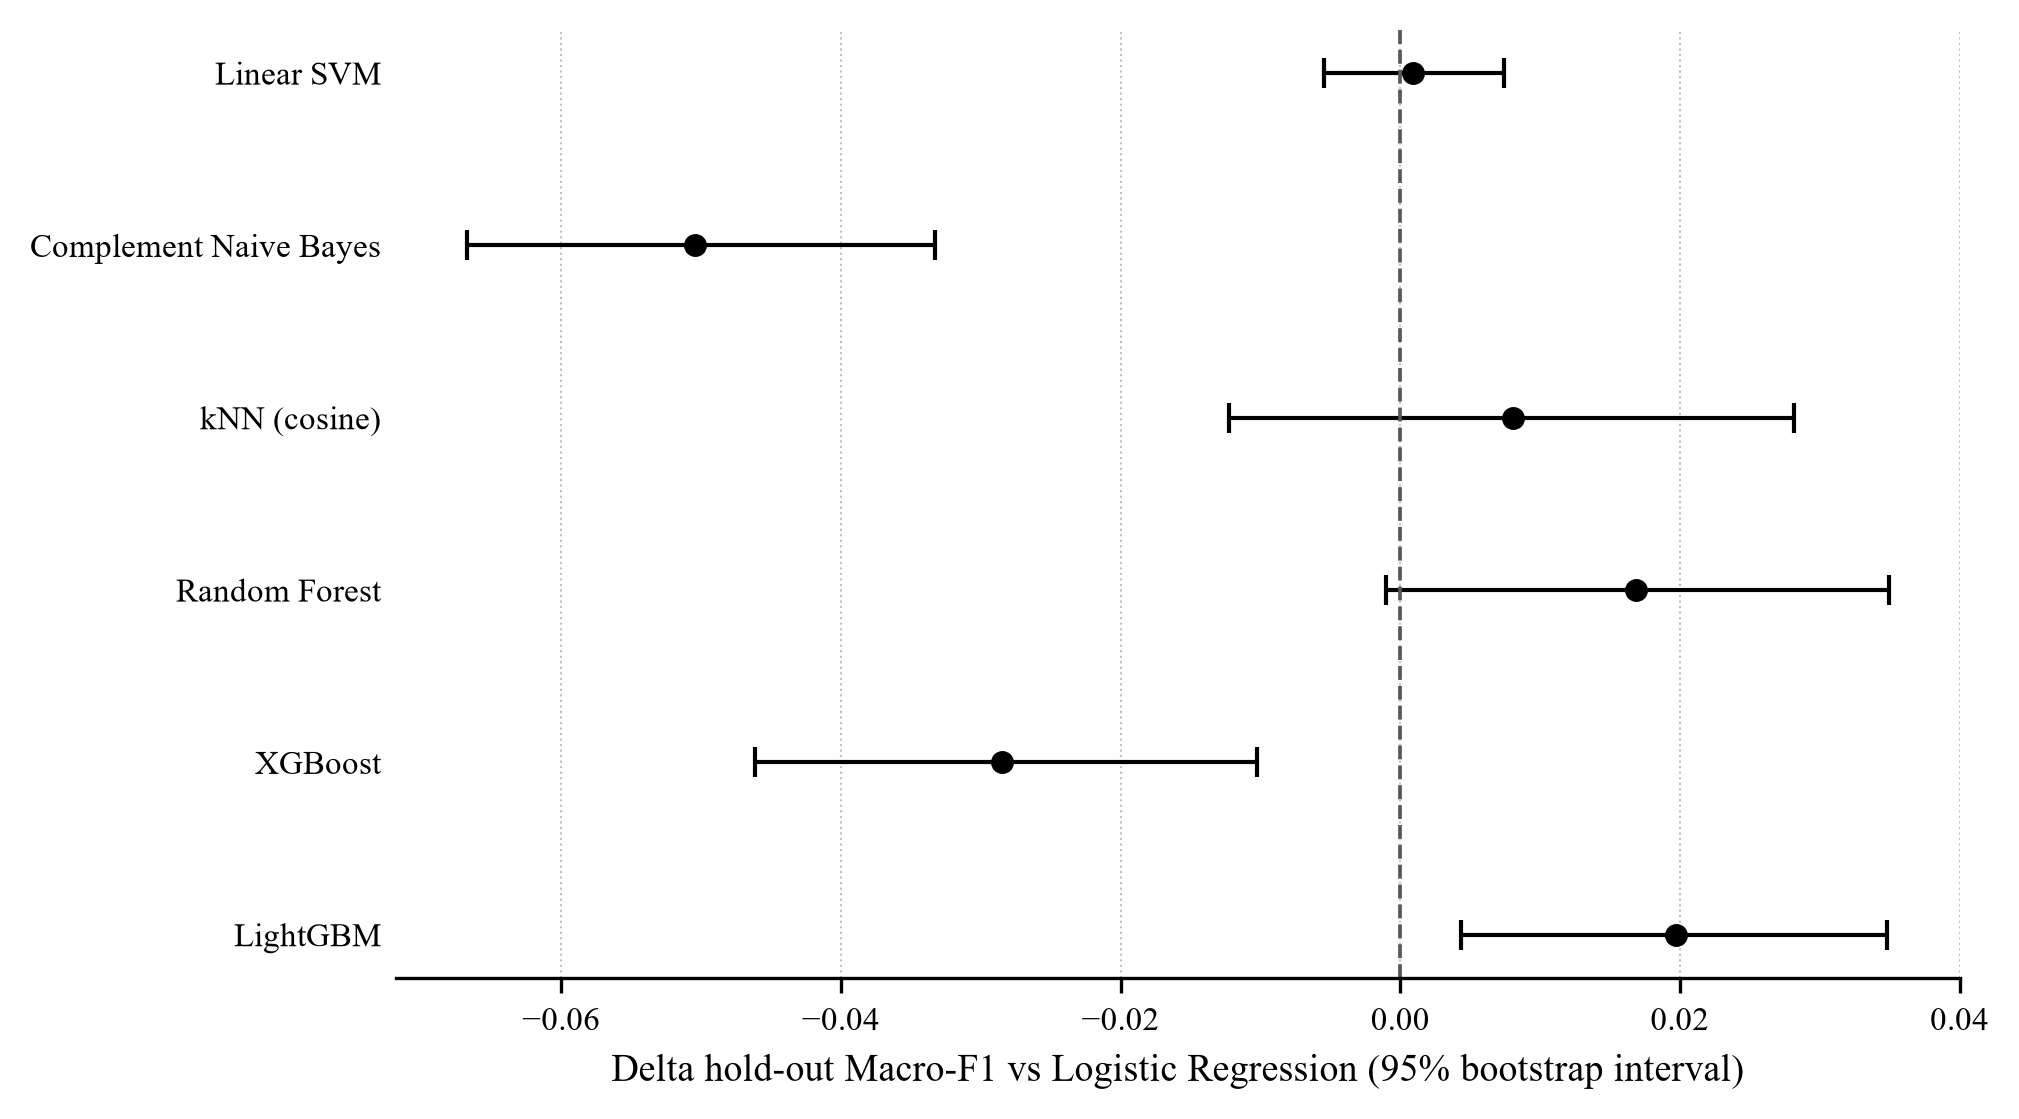
\includegraphics[width=\linewidth]{figures/04_H1_pairwise_macro_f1_differences.png}
\caption{Pairwise differences in Macro-F1 between the alternative classifiers
and the Logistic Regression baseline on FS4.}
\Description{Forest plot comparing six alternative classifiers with Logistic
Regression on FS4. LightGBM has a positive confidence interval entirely above
zero. Random Forest and kNN have positive point estimates with intervals
crossing zero, Linear SVM is close to zero, and XGBoost and Complement Naive
Bayes show negative differences.}
\label{fig:h1_pairwise}
\end{figure}

For LightGBM, a positive difference of
$\Delta F1_{\mathrm{macro}} = 0.0197$ was obtained. The 95\% confidence
interval was entirely above zero, 95\% CI [0.0044, 0.0348], and the
directional comparison remained statistically significant after Holm
correction for multiple testing ($p_{\mathrm{Holm}} = 0.024$).

A positive difference was also observed for Random Forest
($\Delta F1_{\mathrm{macro}} = 0.0169$), although the 95\% CI
[$-0.0010$, 0.0350] included zero, and the difference was not statistically
significant after Holm correction ($p_{\mathrm{Holm}} = 0.161$). No
statistically significant improvements over the baseline were found for kNN
($\Delta F1_{\mathrm{macro}} = 0.0081$, 95\% CI [$-0.0122$, 0.0282],
$p_{\mathrm{Holm}} = 0.855$) or Linear SVM
($\Delta F1_{\mathrm{macro}} = 0.0009$, 95\% CI [$-0.0054$, 0.0074],
$p_{\mathrm{Holm}} = 1.000$). For XGBoost
($\Delta F1_{\mathrm{macro}} = -0.0285$, 95\% CI
[$-0.0462$, $-0.0103$]) and Complement Naive Bayes
($\Delta F1_{\mathrm{macro}} = -0.0504$, 95\% CI
[$-0.0668$, $-0.0333$]), the observed effects were entirely in the opposite
direction.

Since at least one of the six prespecified comparisons showed a positive
effect that remained statistically significant after Holm correction, H1 is
supported.

The final model selected based on cross-validation was LightGBM with feature
set FS5. It achieved a mean cross-validation Macro-F1 of 0.5330
(SD = 0.0097) and a Macro-F1 of 0.5597 on the separate hold-out dataset
(95\% CI [0.5431, 0.5757]).

At the class level, the final FS5-LightGBM model achieved a Precision of
0.6457, a Recall of 0.6819, and an F1 score of 0.6633 for high-priority
tickets. For the medium-priority class, Precision was 0.5577, Recall was
0.6471, and F1 was 0.5991. The lowest class-specific performance was observed
for low-priority tickets, with a Precision of 0.5674, a Recall of 0.3291, and
an F1 score of 0.4166. Low-priority tickets were most frequently confused with the medium-priority class, whereas medium- and high-priority tickets were classified correctly more often. The corresponding class-specific prediction pattern is
shown in the normalized confusion matrix (see Figure~\ref{fig:final_confusion_matrix}). 

\begin{figure}[ht]
\centering
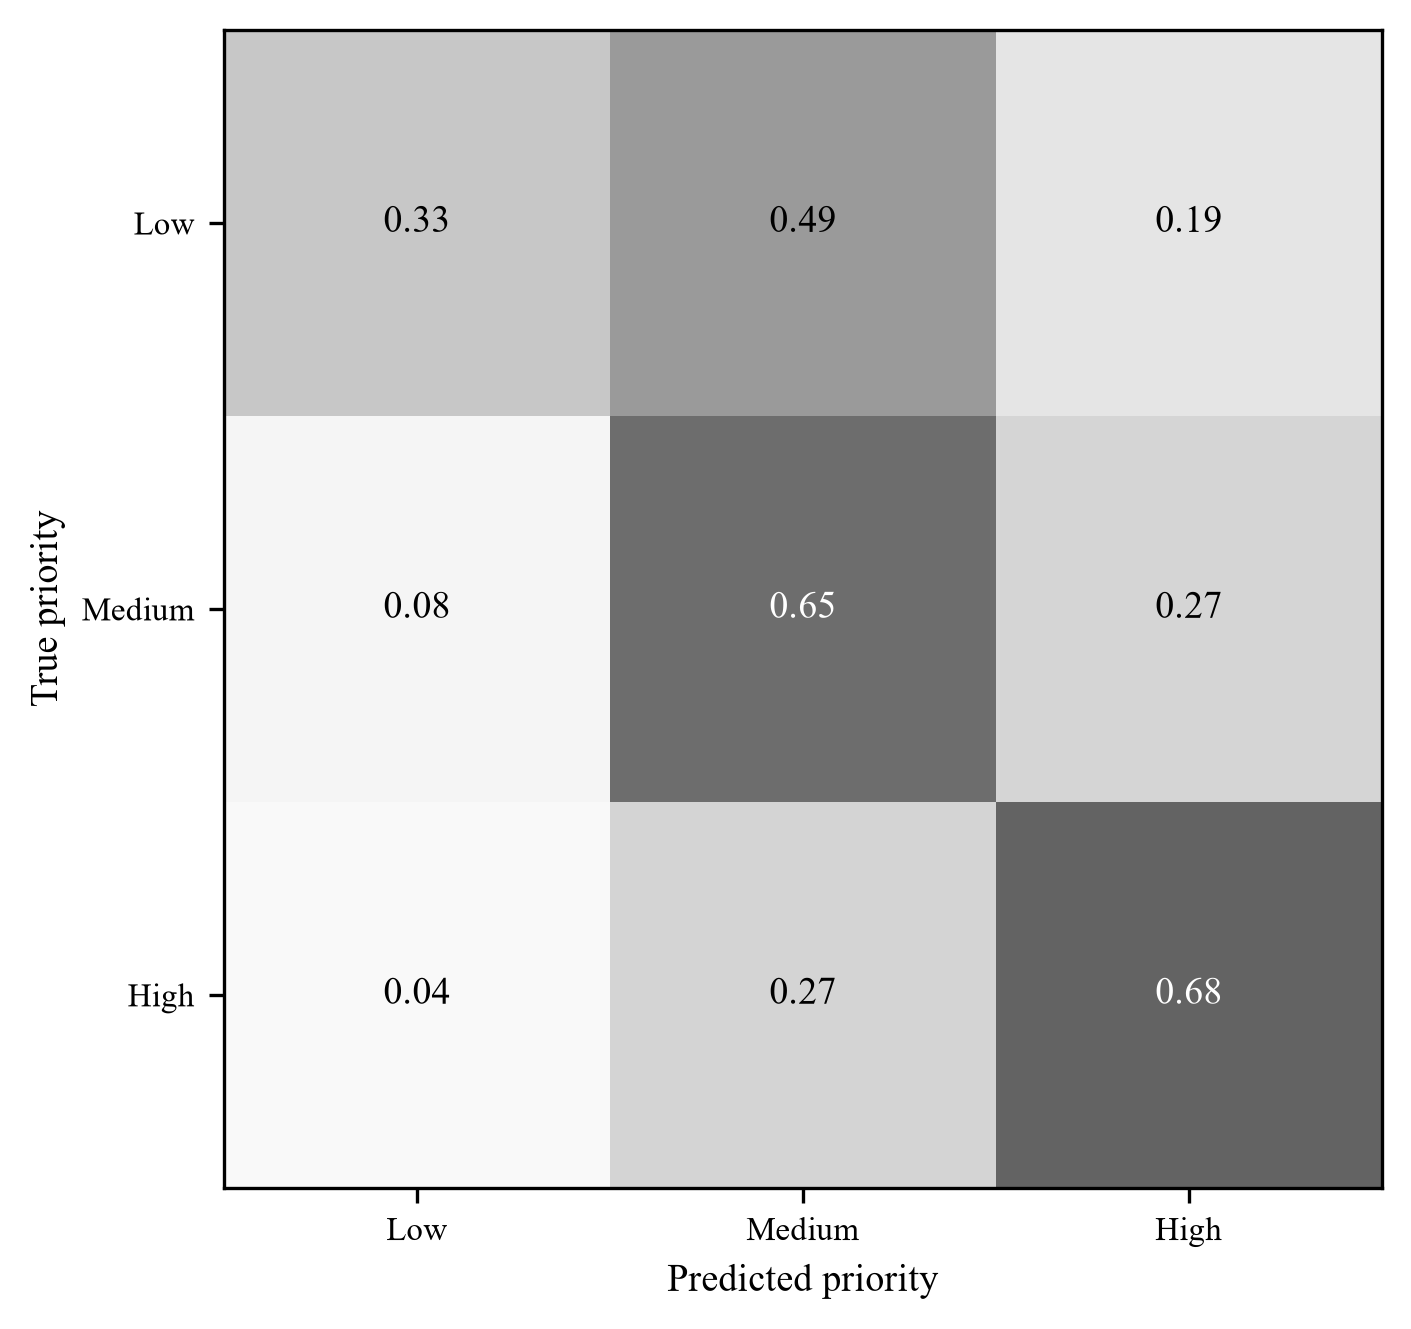
\includegraphics[width=0.72\linewidth]{figures/04_final_model_confusion_matrix.png}
\caption{Normalized confusion matrix of the final FS5-LightGBM model on the
hold-out dataset.}
\Description{Three-by-three row-normalized confusion matrix. Low-priority
tickets are predicted as low, medium, and high with proportions 0.33, 0.49,
and 0.19. The corresponding proportions are 0.08, 0.65, and 0.27 for
medium-priority tickets and 0.04, 0.27, and 0.68 for high-priority tickets.}
\label{fig:final_confusion_matrix}
\end{figure}

\subsection{SHAP-Based Explainability and Attribution Patterns}

The SHAP-based explanation compactness of the seven classifiers was examined
on the common feature set FS4 based on the concentration of absolute SHAP
attributions. The primary measure was Top-10 concentration, defined as the
proportion of the total absolute SHAP mass attributable to the ten features
with the highest absolute attributions. Higher values correspond to a stronger
concentration of the attributions on a small number of features. Figure~\ref{fig:h2_compactness} shows the Top-10 concentration of absolute SHAP mass across the
common explainability sample.

\begin{figure}[ht]
\centering
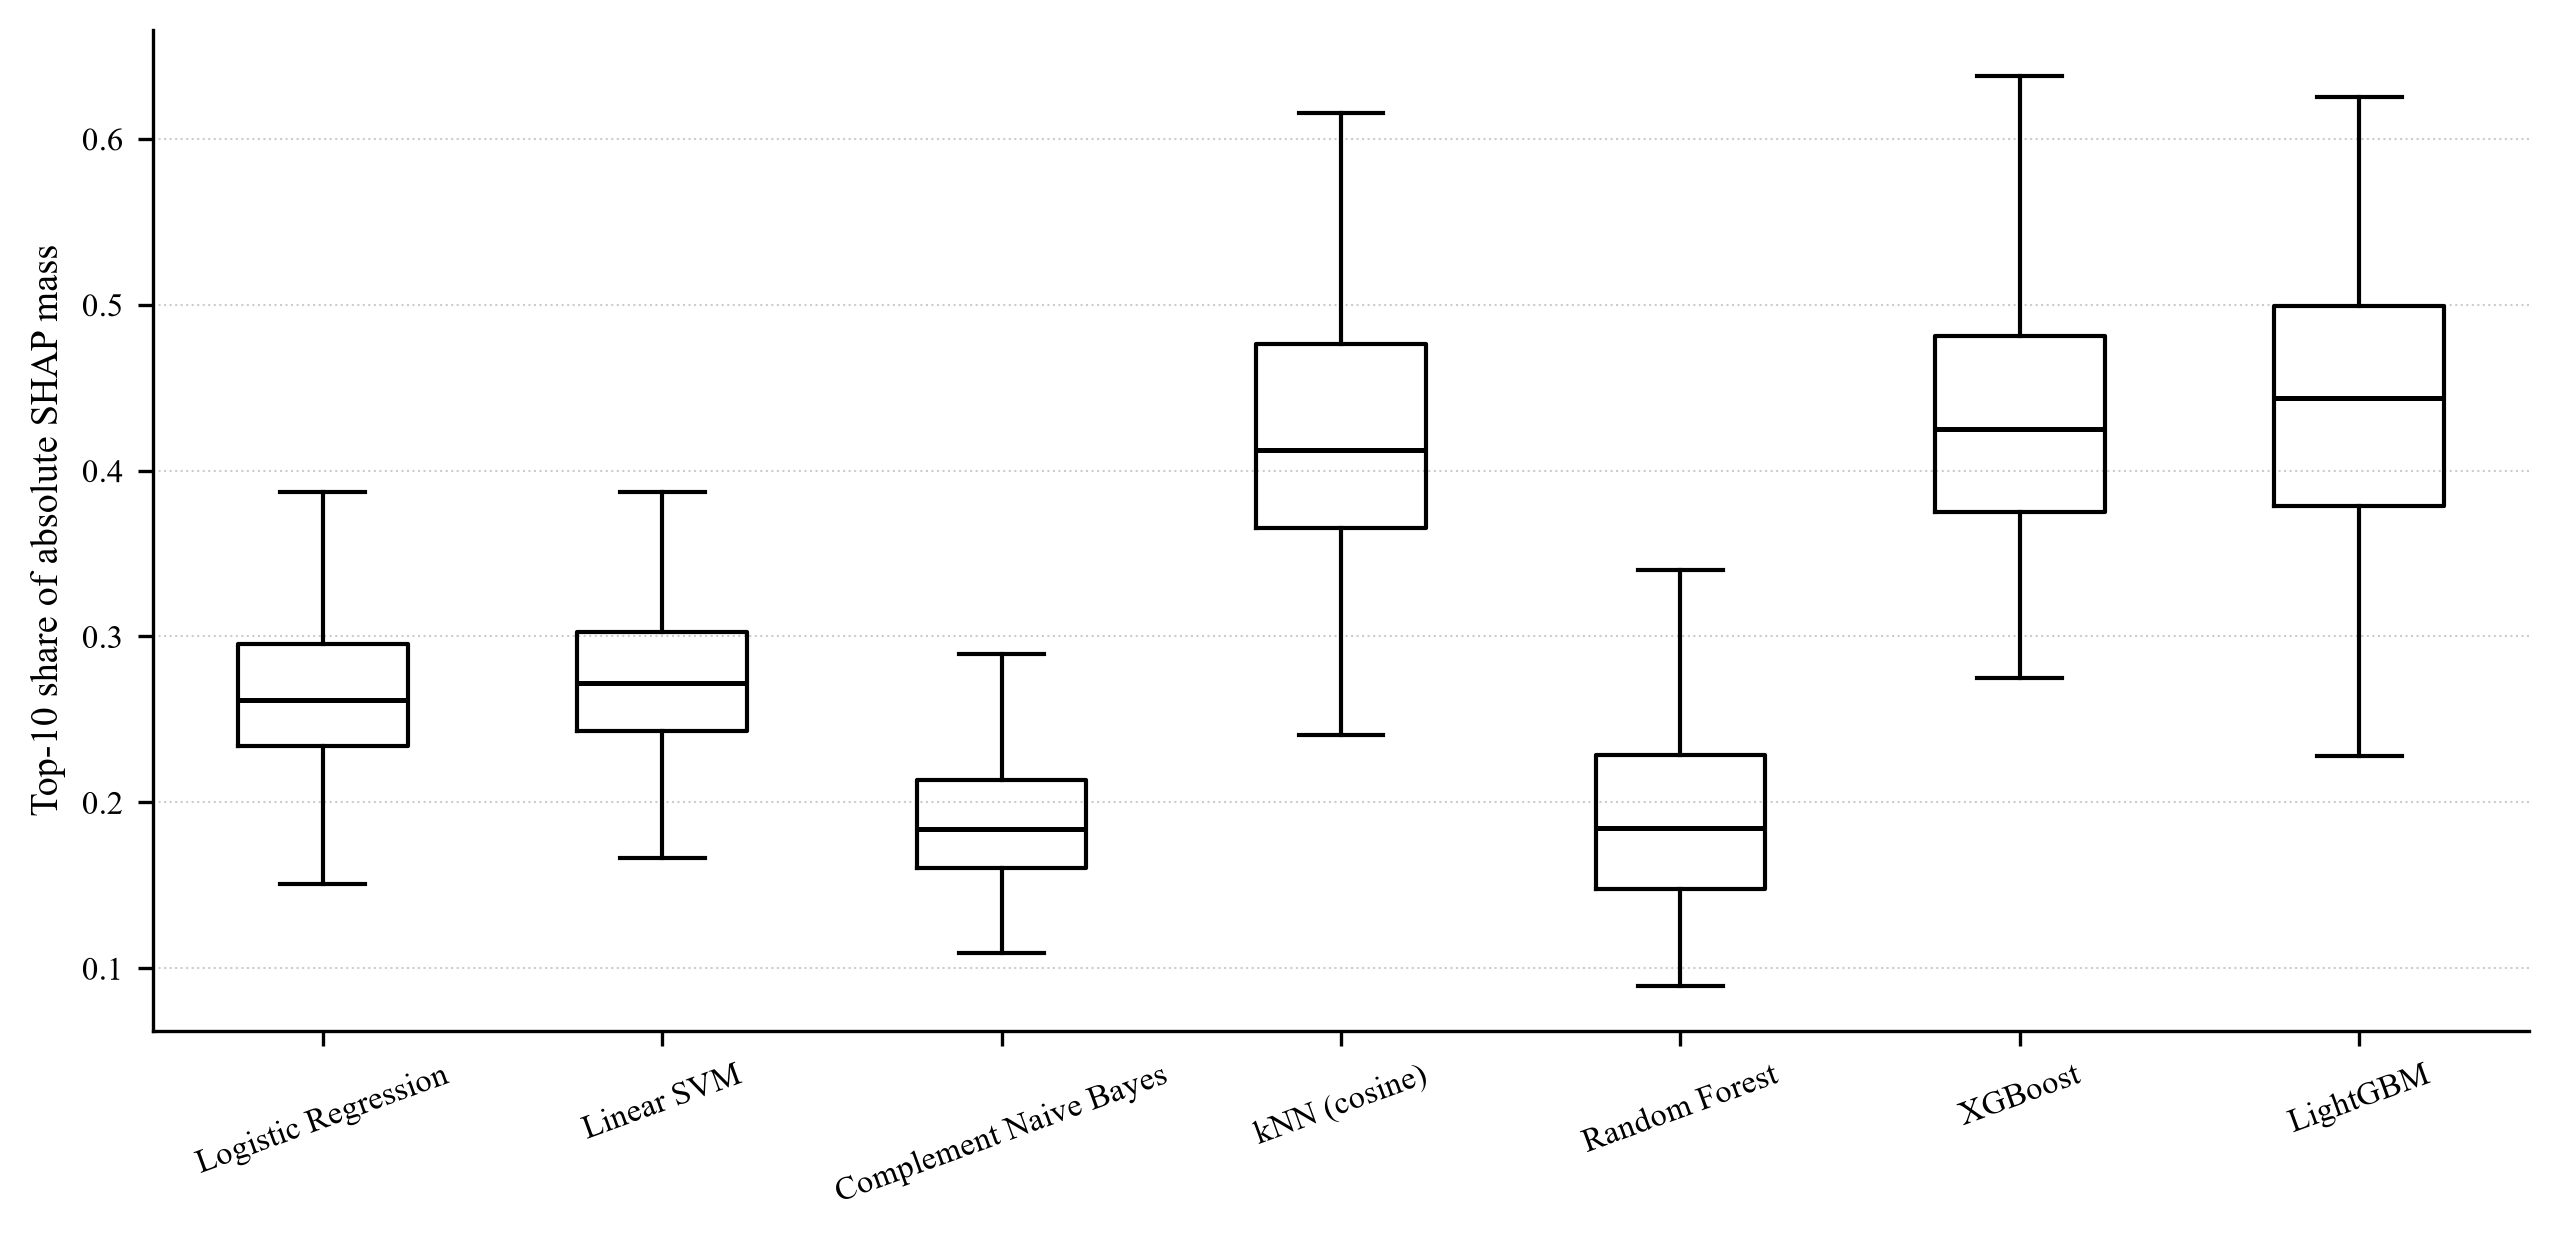
\includegraphics[width=\linewidth]{figures/05_h2_compactness_by_model.png}
\caption{SHAP-based explanation compactness of the seven classifiers on FS4.}
\Description{Boxplots of Top-10 absolute SHAP-mass concentration for the seven
classifiers. Complement Naive Bayes and Random Forest show the lowest
concentrations, Logistic Regression and Linear SVM intermediate values, and
kNN, XGBoost, and LightGBM substantially higher concentrations.}
\label{fig:h2_compactness}
\end{figure}

The mean Top-10 concentration was 0.2657 for Logistic Regression and 0.2740
for Linear SVM. Lower values were observed for Complement Naive Bayes
(0.1882) and Random Forest (0.1916). Higher concentrations were obtained for
kNN (0.4238), XGBoost (0.4286), and LightGBM (0.4388).

To test H2, the pairwise differences in Top-10 concentration were calculated
according to Equation~\ref{eq:h2_delta}. Positive values indicate higher
explanation compactness for Logistic Regression. For Complement Naive Bayes,
the difference was $\Delta \mathrm{Top10} = 0.0775$. The 95\% CI
[0.0727, 0.0823] was entirely above zero, and the Holm-corrected directional
test was statistically significant ($p_{\mathrm{Holm}} < 0.001$). Logistic
Regression also showed a significantly higher Top-10 concentration than
Random Forest ($\Delta \mathrm{Top10} = 0.0741$, 95\% CI
[0.0676, 0.0805], $p_{\mathrm{Holm}} < 0.001$).

For Linear SVM, in contrast, the difference was
$\Delta \mathrm{Top10} = -0.0083$, 95\% CI
[$-0.0106$, $-0.0062$]. The confidence intervals were also entirely below
zero for kNN ($\Delta \mathrm{Top10} = -0.1582$, 95\% CI
[$-0.1670$, $-0.1489$]), XGBoost
($\Delta \mathrm{Top10} = -0.1630$, 95\% CI
[$-0.1700$, $-0.1558$]), and LightGBM
($\Delta \mathrm{Top10} = -0.1731$, 95\% CI
[$-0.1831$, $-0.1632$]). The directional comparisons were not statistically
significant in these cases.

Since at least one of the six prespecified comparisons showed a positive
effect that remained statistically significant after Holm correction, H2 is
supported. This criterion was met for Complement Naive Bayes and Random
Forest. At the same time, the results show that Logistic Regression did not
exhibit higher explanation compactness than all investigated classifiers.

The robustness analyses confirmed the H2 pattern for Complement Naive Bayes
across all five investigated operationalizations. For Random Forest, the
advantage of Logistic Regression was observed for Top-5 concentration,
Top-20 concentration, and Top-10 concentration restricted to active features,
but not for \(K_{80}\) or normalized entropy. The result for Random Forest was
therefore dependent on the measure used.

The complementary faithfulness analysis showed that removing the ten active
text features with the highest absolute SHAP values resulted in a larger
decrease in the score of the originally predicted class than removing the same
number of randomly selected active text features in more than half of the
cases for all seven classifiers. The corresponding proportion ranged from
60.67\% for XGBoost to 98.67\% for Complement Naive Bayes. For Logistic
Regression, the proportion was 82.67\%, compared with 72.00\% for LightGBM.
For XGBoost, the comparison between approximate and exact SHAP contributions
yielded a high rank correlation.

The class-switch rate was also higher for all seven classifiers after removal
of the ten most important SHAP text features than after removal of randomly
selected active text features. Following SHAP-based removal, class-switch
rates ranged from 0.1600 to 0.4200, compared with 0.0400 to 0.1173 following
random removal.

In addition, the finally selected FS5-LightGBM model was analyzed separately
using SHAP. With respect to the predicted class in each case, 82.33\% of the
total absolute SHAP mass was attributable to text features and 15.63\% to the
ticket queue. Ticket type accounted for 1.10\%, sentiment features for
0.94\%, and language for less than 0.01\%. At the class level, the proportion
attributable to text features was 80.17\% for low priority, 90.23\% for
medium priority, and 75.34\% for high priority. The corresponding proportions
attributable to the queue were 18.56\%, 8.95\%, and 20.92\%.

The qualitative plausibility assessment of the twelve local comparison cases
yielded a heterogeneous picture. While some of the SHAP explanations were
considered plausible in terms of their content, others were rated as only
partially plausible or not plausible, particularly when the attributions were
dominated by features with limited discriminative value or features that were
difficult to interpret.
\section{Discussion}

This section interprets the empirical findings with respect to the research
questions and the existing literature. The limitations of the study are then
discussed, followed by implications for future research and potential
application scenarios.

\subsection{Interpretation of Classification Performance and Explainability}

RQ1 examined how the investigated ML classifiers differ in performance for
NLP-based prioritization of IT support tickets. On the common data, split, and
feature basis, LightGBM achieved the highest hold-out Macro-F1 on FS4 and was
the only alternative that significantly outperformed Logistic Regression after
Holm correction. The observed difference was
$\Delta F1_{\mathrm{macro}} = 0.0197$, which supports H1. This does not
indicate a general superiority of more complex model families. Earlier ticket
studies likewise report context-dependent rankings, with different models
performing best across datasets and classical SVM approaches remaining
competitive with more complex methods
\cite{ahmed2023incident,martins2024port,bonechi2024support}.

The feature basis also affected performance. FS4 achieved the highest average
cross-validation performance across all seven classifiers, indicating that
queue information added predictive value in this dataset. The SHAP analysis
of the final model also assigned a relevant share of attribution mass to the
queue. This is consistent with work that incorporates ticket-related and
contextual information in addition to text
\cite{beckers2009multifacet,fuchs2022support}. Queue structures are tied to
organizational processes, so this predictive value may not transfer directly
to other service organizations. Sentiment features added little.
FS5-LightGBM reached a hold-out Macro-F1 of 0.5597 compared with 0.5594 for
FS4-LightGBM, while sentiment accounted for less than one percent of absolute
SHAP mass.

The final model should not be interpreted as ready for immediate production
use. Low-priority tickets were identified less reliably, with a Recall of
0.3291, and Macro-F1 does not reflect different operational consequences of
misclassification. The moderate classification performance may partly reflect the information
available for priority prediction, as \citet{tian2015priority} model
bug-report priority as a multi-factor decision involving textual, temporal,
author, related-report, severity, and product information. In contrast, the
present study was restricted to the text and structured features available in
the investigated dataset. In addition, real-world ITSM research reports
particular difficulties for semantically complex and underrepresented classes
\cite{razma2026classification}. RQ1 is therefore answered by the finding that the
classifiers differed in prioritization performance. LightGBM performed best
on the common feature basis and was the only alternative with a statistically
significant advantage over Logistic Regression, while no general superiority
of more complex model families was observed.

RQ2 examined differences in SHAP-based explanation properties. Explanation
compactness was operationalized for inferential testing. Logistic Regression
showed significantly higher Top-10 concentration than Complement Naive Bayes
and Random Forest, which supports H2 under the prespecified criterion. No such
advantage was observed over Linear SVM, kNN, XGBoost, or LightGBM.
Robustness analyses confirmed the result for Complement Naive Bayes across all
five operationalizations, whereas the comparison with Random Forest depended
on the compactness measure used.

These findings extend earlier XAI work in ticket classification. Local
explanation methods have been used to analyze relevant features and
misclassifications, while SHAP-based explanations have been integrated into
helpdesk systems \cite{zicari2022ticket,licina2026helpagent}. In contrast to studies that primarily evaluate ticket-classification performance
or use explanations within individual classification frameworks \cite{razma2026classification,zicari2022ticket,licina2026helpagent}, the present
analysis compares SHAP-based explanation compactness across the investigated
classifiers. This comparison shows that predictive performance and explanation compactness
do not follow a consistent trade-off. Explanation quality is multidimensional
\cite{nauta2023evaluation}, so faithfulness and robustness were considered in
addition to compactness. The faithfulness analysis indicated that highlighted
features were related to model behavior, while local cases showed
heterogeneous plausibility. SHAP describes feature attributions to model predictions
\cite{lundberg2017shap}, which should not be interpreted as establishing
causal relationships \cite{janzing2020causal}. Comprehensibility for
actual users was not examined systematically, so the findings do not replace
independent user or expert evaluation. RQ2 is therefore answered by
model-dependent differences in SHAP-based explanation properties without a
consistent advantage of Logistic Regression or a simple separation between
linear and more complex models.

\subsection{Limitations}

A central limitation is the synthetic data basis. Public availability supports
reproducible comparison \cite{bueck2025support}. Synthetic data may not fully
capture characteristics and distributions observed in real-world data
\cite{goyal2024synthetic}. In the present context, this concerns in particular
language, support processes, and error patterns and may therefore limit
transferability to real ITSM environments. The dataset also includes broader queues such as
Human Resources, Sales and Pre-Sales, and General Inquiry. The findings
therefore concern a heterogeneous support population rather than a narrowly
defined IT service desk.

The analysis assumed that the queue was already available when priority was
predicted. Because no process timestamps establish the order of queue and
priority assignment, this assumption could not be verified. Priority and
language labels could not be validated independently. Manual reviews assessed
the plausibility of data-quality decisions rather than reassigning priorities.
Semantic grouping also depends on the Sentence-BERT representation, the
similarity threshold of 0.95, and the complete-linkage strategy
\cite{reimers2019sentencebert}.

The group-based hold-out measures generalization within the same dataset.
Neither external nor temporal validation was conducted. This is relevant because
model performance in IT-related classification has been shown to depend on the
application context \cite{ahmed2023incident}, while temporal changes may alter
the relationship between input data and target concepts \cite{gama2014conceptdrift}.
Consequently, concept drift, alternative queue structures, and
organization-specific prioritization rules remain unobserved. The algorithm and representation screenings were exploratory and budget-limited. Hyperparameters selected on FS1 were fixed for later feature-set comparisons. This improves comparability but may prevent individual
models from reaching their optimum on later feature sets. The cross-validation
Macro-F1 of 0.5330 therefore represents model-selection performance within the
training partition, while the hold-out Macro-F1 of 0.5597 represents the
separate final evaluation.

Different model structures required different SHAP explainers, which limits
the direct comparability of the H2 results across models. Because
Shapley-based attributions can vary depending on how they are computed
\cite{sundararajan2020many}, the observed H2 differences in explanation
compactness may reflect both model differences and differences in the
attribution method. The H2 sample contained 100 semantic
groups per priority class, giving all classes equal weight rather than their
natural frequencies. Random Forest and XGBoost were explained approximately
for computational reasons. Exact and approximate XGBoost attributions showed
high agreement with $\rho = 0.9666$, but this cannot be assumed for Random
Forest. The kNN explanations were sensitive to the background sample and
evaluation budget. The qualitative plausibility assessment was conducted by the author rather
than independent ITSM experts. Since explanation quality is multidimensional
\cite{nauta2023evaluation}, the present analysis cannot establish whether the
explanations are understandable or decision-relevant for ITSM practitioners.

\subsection{Implications and Future Research}

The findings suggest that automated ticket prioritization can benefit from
structured contextual information in addition to text. More complex
classifiers did not consistently outperform the baseline, so a
supportive human-in-the-loop setting appears more plausible initially than
fully autonomous priority assignment. This approach was also adopted in prior work
on intelligent ticket management \cite{zicari2022ticket}.

Future studies should test the findings on real-world ITSM data across multiple
organizations and use temporal test sets. Cost-sensitive or ordinal learning
objectives could better reflect unequal operational consequences of errors.
The exploratory transformer screening could also be extended by evaluating
multilingual transformer classifiers such as XLM-RoBERTa (XLM-R) \cite{conneau2020xlmr}
under the full group-based modeling and hold-out design. Independent assessments
by ITSM experts would complement model-based XAI metrics by examining
comprehensibility and actual decision utility.

Overall, the study provides a controlled comparison of classifiers and their SHAP-based explanations under a common evaluation design. Whether the observed technical differences translate into operational value requires subsequent real-world process and user evaluation.
\section{Conclusion}

This study examined the automatic prioritization of IT support tickets using
NLP and machine learning together with the SHAP-based explainability of the
resulting model predictions. Seven classifiers were compared under a common
group-based evaluation design and assessed with respect to classification
performance and selected explanation properties.

RQ1 shows that the investigated classifiers differed in their prioritization
performance, although no general superiority of a particular model family was
observed. On FS4, which was selected as the common feature set based on
cross-validation, LightGBM achieved the highest hold-out performance and was
the only alternative that significantly outperformed Logistic Regression after
Holm correction. H1 is therefore supported. The final model selected overall
was LightGBM with FS5, which achieved a Macro-F1 of 0.5597 on the separate
hold-out dataset. In addition to the ticket text, the queue provided relevant
contextual information, whereas the additional contribution of sentiment
features was small.

RQ2 also revealed clear model-dependent differences. Logistic Regression
showed significantly higher SHAP-based explanation compactness than Complement
Naive Bayes and Random Forest, but not than all alternative classifiers. H2 is
therefore supported according to the prespecified criterion. At the same time,
LightGBM combined comparatively high classification performance with a high
concentration of SHAP attributions. The results consequently provide no
evidence of a consistent trade-off between predictive performance and
explanation compactness.

The interpretation of these findings is mainly limited by the synthetic data
basis, the absence of independent validation of the priority labels, and the
evaluation within a single dataset. Further limitations arise from the
organization-specific role of the queue and from methodological constraints
of the SHAP-based model comparisons. The findings should therefore be
understood as a controlled comparison of the investigated approaches rather
than as evidence of readiness for operational deployment.

Future research should replicate the analysis on real-world ITSM data,
preferably across multiple organizations, and use temporal test sets to examine
concept drift. Ordinal and cost-sensitive learning approaches may offer useful
extensions, as may multilingual transformer-based models such as
XLM-R \cite{conneau2020xlmr}. Explainability research should also examine whether the
identified SHAP explanations are perceived by ITSM experts as understandable
and relevant to decision making. A subsequent field study could then assess
whether model-supported prioritization in a human-in-the-loop setting leads to
measurable improvements in operational service metrics.

\printbibliography

\appendix

\section{Supplementary Materials}

\textbf{Code}\quad
\url{https://github.com/verenagraef/Ticket_Prioritization}

\section{Use of Generative AI}

Generative AI tools were used in a supporting role during manuscript
preparation and code quality assurance. The specific uses are summarized in
Table~\ref{tab:ai-use}.

\begin{table}[ht]
\caption{Use of generative AI tools during the study.}
\label{tab:ai-use}
\begin{tabular}{p{0.18\linewidth} p{0.34\linewidth} p{0.40\linewidth}}
\toprule
Tool & Purpose & Use and verification \\
\midrule
ChatGPT
& Language quality assurance and translation support
& Used to support linguistic revision of manuscript text and the translation
of author-written passages from German into English. Suggested formulations
were reviewed and revised by the author before inclusion in the manuscript. \\

Claude
& Code review
& Used to support the review of Python code with respect to code structure,
consistency, and potential implementation issues. Suggested changes were
evaluated by the author before being applied. \\
\bottomrule
\end{tabular}
\end{table}

\section{Reproducibility Checklist for JAIR}

\subsection*{All articles:}

%\hh{revised for stylistic consistency:}
\begin{enumerate}
    \item All claims investigated in this work are clearly stated. 
    [yes]
    \item Clear explanations are given how the work reported substantiates the claims. 
    [yes]
    \item Limitations or technical assumptions are stated clearly and explicitly. 
    [yes]
    \item Conceptual outlines and/or pseudo-code descriptions of the AI methods introduced in this work are provided, and important implementation details are discussed. 
    [NA]
    \item 
    Motivation is provided for all design choices, including algorithms, implementation choices, parameters, data sets and experimental protocols beyond metrics.
    [yes]
\end{enumerate}

\subsection*{Articles containing theoretical contributions:}
Does this paper make theoretical contributions? 
[no] 

\subsection*{Articles reporting on computational experiments:}
Does this paper include computational experiments? [yes]

If yes, please complete the list below.
\begin{enumerate}
    \item 
    All source code required for conducting experiments is included in an online appendix 
    or will be made publicly available upon publication of the paper.
    The online appendix follows best practices for source code readability and documentation as well as for long-term accessibility.
    [yes]
    \item The source code comes with a license that
    allows free usage for reproducibility purposes.
    [yes]
    \item The source code comes with a license that
    allows free usage for research purposes in general.
    [yes]
    \item 
    Raw, unaggregated data from all experiments is included in an online appendix 
    or will be made publicly available upon publication of the paper.
    The online appendix follows best practices for long-term accessibility.
    [yes]
    \item The unaggregated data comes with a license that
    allows free usage for reproducibility purposes.
    [yes]
    \item The unaggregated data comes with a license that
    allows free usage for research purposes in general.
    [yes]
    \item If an algorithm depends on randomness, then the method used for generating random numbers and for setting seeds is described in a way sufficient to allow replication of results. 
    [yes]
    \item The execution environment for experiments, the computing infrastructure (hardware and software) used for running them, is described, including GPU/CPU makes and models; amount of memory (cache and RAM); make and version of operating system; names and versions of relevant software libraries and frameworks. 
    [yes]
    \item 
    The evaluation metrics used in experiments are clearly explained and their choice is explicitly motivated. 
    [yes]
    \item 
    The number of algorithm runs used to compute each result is reported. 
    [yes]
    \item 
    Reported results have not been ``cherry-picked'' by silently ignoring unsuccessful or unsatisfactory experiments. 
    [yes]
    \item 
    Analysis of results goes beyond single-dimensional summaries of performance (e.g., average, median) to include measures of variation, confidence, or other distributional information. 
    [yes]
    \item 
    All (hyper-) parameter settings for 
    the algorithms/methods used in experiments have been reported, along with the rationale or method for determining them. 
    [yes]
    \item 
    The number and range of (hyper-) parameter settings explored prior to conducting final experiments have been indicated, along with the effort spent on (hyper-) parameter optimisation. 
    [yes]
    \item 
    Appropriately chosen statistical hypothesis tests are used to establish statistical significance
    in the presence of noise effects.
    [yes]
\end{enumerate}


\subsection*{Articles using data sets:}
Does this work rely on one or more data sets (possibly obtained from a benchmark generator or similar software artifact)? 
[yes]

If yes, please complete the list below.
\begin{enumerate}
    \item 
    All newly introduced data sets 
    are included in an online appendix 
    or will be made publicly available upon publication of the paper.
    The online appendix follows best practices for long-term accessibility with a license
    that allows free usage for research purposes.
    [NA]
    \item The newly introduced data set comes with a license that
    allows free usage for reproducibility purposes.
    [yes]
    \item The newly introduced data set comes with a license that
    allows free usage for research purposes in general.
    [yes]
    \item All data sets drawn from the literature or other public sources (potentially including authors' own previously published work) are accompanied by appropriate citations.
    [yes]
    \item All data sets drawn from the existing literature (potentially including authors’ own previously published work) are publicly available. [yes]
    %\item All data sets that are not publicly available are described in detail.
    %[NA]
    \item All new data sets and data sets that are not publicly available are described in detail, including relevant statistics, the data collection process and annotation process if relevant.
    [NA]
    \item 
    All methods used for preprocessing, augmenting, batching or splitting data sets (e.g., in the context of hold-out or cross-validation)
    are described in detail. [yes]
\end{enumerate}

\end{document}